% !TEX TS-program = xelatex
% !TeX program = xelatex
% !TEX encoding = UTF-8
% !TEX spellcheck = en-US
\documentclass[12pt, oneside, a4paper]{article}
%\usepackage{fullpage}
\usepackage[left=2.5cm,right=1.5 cm,top=1.5 cm,bottom=1.5 cm]{geometry}
\usepackage{amsmath,amssymb}             % AMS Math
\usepackage[T1]{fontenc}
\usepackage[utf8]{inputenc}
\usepackage[french,english]{babel}
\usepackage{txfonts} 
\usepackage[]{graphicx}
\usepackage{multirow}
\usepackage{hyperref}
\usepackage{natbib}
\usepackage{indentfirst}


\renewcommand{\baselinestretch}{1.25}

%======================================================
\DeclareMathOperator{\ssfgc}{\textit{SSF-GC}}
\DeclareMathOperator{\ord}{\textit{ord}}
\DeclareMathOperator{\iord}{\textit{iord}}
\DeclareMathOperator{\simil}{\textit{sim}}
\DeclareMathOperator{\nextsent}{\textit{next}}
\DeclareMathOperator{\lastsent}{\textit{last}}
\DeclareMathOperator{\tfisf}{\textit{tf-isf}}
\DeclareMathOperator{\tfidf}{\textit{tf-idf}}
%======================================================


\begin{document}

%\selectlanguage {francais}
\pagenumbering{arabic}

%\twocolumn[%
%\begin{@twocolumnfalse}
%\maketitle
\noindent

\includegraphics[width=\textwidth]{figures/logo/esi-header.png}

\noindent
Abdelkrime Aries  \\
\'Ecole doctorale STIC 2010 \\
LCSI laboratory\\
\noindent
\begin{tabular}{@{}ll}
Supervisors: & Djamal Eddine Zegour \\
& Walid Khaled Hidouci\\
\end{tabular}\\[.5 cm]

\noindent
\begin{center}
	Thesis report (Summary)\\
{\LARGE \textbf{Vers une amélioration \\des résumés automatiques de textes}}\\[.5 cm]
{\large\itshape Towards improving automatic text summaries}\\[1 cm]
\end{center}
%\end{@twocolumnfalse}
%]

\section{Introduction}

We live in the age of data, where a huge mass of information is produced everyday. 
It can be found in many sources, such as electronic newspapers, with many variations.
The redundant information makes their selection and processing very difficult.
One way to ease this task is using automatic text summarization (ATS).

\subsection{Summarization challenges}

There exists a lot of challenges which harden the advance of ATS. 
One of these problems is the absence of a precise definition of what should be included in a summary. 
Over time, several works were conducted to generate the perfect summary which must be informative on one hand, and not redundant on the other. 

Summary's informativeness is another challenge to tackle.
The main goal of a summary is to afford a representative text of the original document. 
It must cover the essential information using few words. 
That means, the summary must retain more information (summary's coverage) with less redundancy (summary's conciseness).

Mostly, ATS methods aim to generate an informative summary, but when it comes to the summary's readability it is a matter of future work.  


\subsection{Thesis motivation}

Summaries can be very useful in real life applications.
For instance, they can enhance productivity and decision making in term of time.
Recently, multilingual content started to grow considerably, which needs more adaptable methods for languages other than English.
As a result, multilingual text summarization began to receive more attention from research community. 
%In 2011, TAC\footnote{TAC: Text Analysis Conference, \url{https://tac.nist.gov}} workshop included a task called ``MultiLing task", which aims to evaluate language-independent summarization algorithms on a variety of languages \citep{11-giannakopoulos-al}.
%This task evolved in 2013 into a workshop called ``MultiLing workshop" as a community-driven initiative for testing and promoting multilingual summarization methods. 
%Afterwards, the workshop was held in 2015, 2017 and 2019. 
In the light of that, our thesis will present ATS with more focus on multilingual context.


\subsection{Thesis aims}

Motivated by the growth of multilingual content on the web, this thesis will be focused on multilingual ATS.
Multilingualism is the ability to use many languages in a specified task (in our case: ATS).
So, a multilingual method must be isolated from language's structure of the input text. 
By definition, most existing methods can be considered as language-independent. 
When it comes to implementing such method into a system, the general challenges presented earlier can be an issue:
\begin{itemize}
	\item Methods based on simple linguistic properties found in most/all languages such as proper nouns can be seen as language independent.
	However, when it comes to multilingual implementation, we face the problem of finding proper nouns for many languages. 
	\item Machine learning ATS methods can be language-independent.
	The language supported by the system depends on the resources used for its training. 
	The problem with this approach is its use of annotated corpora for each language we want to add. 
	
\end{itemize}

In conclusion, even if a method is language-independent, it can be difficult to adapting the system implementing it into new languages.
In this case, the system can be considered as partially language-independent. 
Our intention is to propose a new method that insures the following conditions:
\begin{itemize}
	\item Simple adaptation: 
	A good multilingual method is the one which can easily be adapted into as many languages as possible. 
	
	\item Informative summaries: 
	A generic method can afford less performance than a language-specific one. 
	So, for a generic method (system) to support many languages with a fair performance is a good method (system). 
	
	\item Coherence: In general, this task needs some language related information to be done properly. 
	In our case, we will focus on sentences ordering.
	
\end{itemize}

\subsection{Report's Outline}

This report is a summary of our thesis. 
We will discuss summarization methods, approaches and evaluation briefly in the first section. 
In the thesis, however, they are discussed in a much detailed manner, where each represents a chapter. 
Then, we will present our participation in MultiLing'15 Workshop with a previous method which we ameliorated to handle multilingual content. 
The 4th section represents our contribution which is a method based on both statistical and graph approaches. 
The next section will discuss our test on how machine learning can perform in a multilingual context. 
Finally, we will finish this report with a conclusion discussing the work that have been done, showing different contributions and opening new discussions for future works.


\section{State of the art review}

We start by presenting the different summarization methods following the taxonomy proposed by \citet{98-hovy-lin,99-sparckjones}. 
Then, 
Our taxonomy is based on the nature of resources used by the method (or the system) since we are more interested on multilingual summarization. 
So, the different approaches presented in this chapter are: statistical, graph-based, linguistic and machine learning. 

\subsection{Summarization methods}

Based on the criteria afforded by \citet{98-hovy-lin} and some other changes to fit current systems, the different classifications can be illustrated as in Figure~\ref{fig:summary-classif}.
A method's categorization can be done based on three criteria: input document, purpose and output document. 
Looking to the input document, we can classify a method based on source size (multi-document, vs. mono-document), specificity (domain-specific vs. general) and form (structure, scale, medium and genre). 
The purpose of a summarization method contains three sub-criteria: audience (query-oriented vs. generic), usage (indicative vs. informative) and expansiveness (background vs. just-the-news).
We changed the definition of the last one (Expansiveness) to fit nowadays methods, this will categorize summaries into background or update.

\begin{figure}[ht]
	\begin{center}
		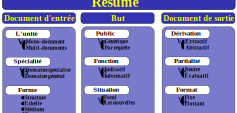
\includegraphics[width=.5\textwidth]{figures/methods/sum-classif.pdf} % % %[width=140mm]
		\caption{Classification of summarization systems using different criteria.}
		\label{fig:summary-classif}
	\end{center}
\end{figure}

% input document 
%=================
Lets start by assessing the impact of the input document categorization on multilingual text summarization. 
% source size
Source size has nothing to do with documents' languages. 
So, if a method is either multi-document or mono-document, this does not affect its multilingualism. 
Of course, if we want to go deep in processing multiple documents using their semantic relationships, in this case a multilingual method can be difficult to set in motion. 
% Specificity
Specificity criterion separates summarization methods into domain-specific and general. 
A domain-specific method uses language resources such as cue words to emphasize a domain over others, which makes it language-dependent. 
On the bright side, being dependent to a domain can help limiting the workload of adapting a certain system to a new language. 
For instance, it is fairly easy to prepare a list of domain words in a certain language, either manually or automatically. 
% form
Summarization systems based on document form are dependent to the structure, scale, medium and genre rather than the input language. 

% purpose
%==========
A summarization method can be categorized according to its purpose based on three criteria: audience, usage and expansiveness.
% Audience
According to the audience criterion a summary can be query-oriented or generic, both can be language independent.
In case of query-oriented methods, there is always a technique to consider users queries without relying on heavy language resources. 
For instance, cosine similarity can be used to calculate the pertinence of a sentence to the query based on their terms. 
% Usage
Looking to the summary's usage, a summary (and the method as well) can be indicative or informative.
An informative summary can be done without relying on heavy language resources. 
As for an indicative summary, if the purpose is to present a little text to invite the reader for reading the whole document, we can apply the  same analogy as informative one. 
If we want to present some information such as ``Who", ``When", ``Why", etc., in this case more language dependent resources are needed.
% Expansiveness
The expansiveness divides summaries into background and update summaries. 
Both of these categories can be generated without relying on heavy language resources.
For instance, in update summaries we can detect novelty using some statistical methods such as cosine similarity.

% Output document
%==========
A summarization method can be categorized according to its output document (the summary) based on three criteria: derivation, usage and expansiveness.
% Derivation
According to derivation, a summarization method can be extractive or abstractive.
The extractive one can rely only on statistical methods to extract some parts of the text, thus it can be language-independent. 
The abstractive, on the other hand, has to use some language information to generate new texts. 
Using Deep learning to produce new texts, the architecture itself is not designed for a specific language. 
But when it comes to the training set, we need a huge amount of text so the system learns a vocabulary and some generation rules. 
%This makes it so hard to adapt the system to many languages and 
% Partiality
According to partiality, a method (or a system) can be neutral or evaluative . 
The latter includes opinion, which can be implicit or explicit. 
Either ways, the system must rely on some language material to detect text opinions in case of implicit summarization, or to understand the text and generate opinions in case of explicit one. 
% Conventionality (Fixed, Floating)
The conventionality criterion, which divides methods into fixed or floating, has no relation with language. 


\subsection{Summarization approaches}

According to \citet{12-nenkova-mckeown}, topic representation approach contains topic words, frequency driven, latent semantic analysis, etc. 
We are, rather, interested in the nature of used resources.
Are they dependent on a specific language? or domain? do the methods need a lot of resources?
This is why we follow their other taxonomy \citep{11-nenkova-mckeown} called ``Semantics and discourse" which we present as ``linguistic approach" since its methods as highly connected to the language being processed.
The taxonomy of \citet{12-lloret-palomar} seems to approach our vision. 
The difference is that we consider topic-based and discourse-based approaches as sub-approaches of linguistic one, since the two are based on linguistic properties of the input text.

Statistical features based methods were the first introduced in ATS. 
Features like term frequency, position and length are language independent and are good indicators of sentence relevance. 
A statistical approach does not need much language dependent tools; just some basic NLP tasks such as sentence segmentation, tokenizaion, stop word elimination, and stemming. 
Mostly, it is easy to be implemented and does not need a lot of processing power.
The statistical features are combined together in hope to better capture a sentence's relevance. 
This leads to a more complicated problem which is how to combine them, and how much amount of influence of each one. 
The problem can be solved by combining them linearly, and set their weights through experiments using a corpus or estimate them using machine learning.
Either way, we will have another problem which is language dependency. 

Graph-based approach seeks to exploit the shared information between sentences. 
It is a bottom-up method which discusses the similarity problem from the perspective of content structure \citep{15-yang-al}. 
It can be language-independent using just lexical similarities (mostly, cosine similarity) and statistical features. 
But, some room for improvement can be done by considering more language dependent similarities such as semantic similarity. 
Also, the model can be improved using machine learning, by introducing prior probabilities into the equation, as in \citep{08-liu-al}.
Processing a great amount of text using iterative graphs can consume more processing power; this should be investigated to better understand how far this approach can go.

Linguistic approach is more powerful than the statistic one in term of expressiveness, because it integrates richer features of the input text. 
Also, it can be used either for extractive or abstractive summarization.  
The problem with this approach is the lack of appropriate NLP tools for certain languages. 
It can be as simple as using sentence components (verbs, nouns, etc.) as statistical features, or as hard as using sentence structure and its relationships with others to generate a new text. 
Mostly, it is harder to be implemented and takes more time to generate a summary. 
\citet{11-nenkova-mckeown} suggests using linguistic methods as a post-processing task to improve linguistic quality of the generated summary rather than a processing one.
According to the authors, it is unclear how much this approach can improve content selection compared to the methods using no linguistic relations. 

All approaches discussed previously can be ameliorated using machine learning (ML).
On the other hand, they can loose multilingual property unless the system is trained on as many languages as possible. 
Still the problem of corpus domain; training your system on news articles does not mean it can handle fiction as good as it does with news.
Also, collecting labeled corpora for one language can be a very hard work, let alone many languages. 
Some works seek to use unlabeled data, and some propose auto-supervised methods such as \citep{02-amini-gallinari}.

\subsection{Summarization evaluation}

Evaluating summarization systems is one of the most difficult tasks. 
Summarization evaluation methods can be intrinsic or extrinsic. 
Intrinsic evaluation is used to judge the performance of a certain method based on the quality of generated summaries.
Basically, the generated summary is compared to a reference one or to the original text in order to test informativeness (coverage and conciseness). 
The summary is also tested based on its readability; whether it contains some unresolved references and if it is coherent.
Extrinsic evaluation evaluates the quality of certain tasks such as information retrieval, reading comprehension and question answering.


In both cases, the evaluation can be manual, automatic or semi-automatic. 
% manual evaluation
In case of manual evaluation, a summary is evaluated by some assessors to judge its quality. 
This type of evaluation excels when it comes to judge if a summary is grammatically correct, if it is coherent, if it performs well for a task, etc.
The dark side of manual evaluation is subjectivity; sometimes the evaluator's experience and point of views can affect their judgment. 
The quality of a good summary can vary from person to another.
Hopefully, there is a solution for this: a summary can be evaluated by many assessors, then the inter-rater agreement between them can be calculated (for example: Kappa coefficient) to verify how well they agree on the score.
Even so, the evaluation can take a long period of time, and the cost of hiring experts to evaluate the summaries can be high. 

% automatic evaluation
On the other hand, automatic evaluation can afford quick results with less or no cost at all. 
In general, it performs well when the evaluation concerns informativeness (coverage and conciseness). 
Many reference summaries of the same document are used in the evaluation since there exists not only one answer but many.
Unfortunately, automatic evaluation methods based on terms or n-grams, such as ROUGE, tend to favor extractive summaries over abstractive ones.
When it comes to readability, automatic evaluation cannot stand a chance against manual one.
Readability, here, refers to references clarity, coherence and grammaticality and not the ease with which a reader can understand a well written text. 
The latter can be measured using automatic metrics such as Flesch–Kincaid readability tests \citep{75-kincaid-al} and SMOG \citep{69-laughlin-harry}.
% semi-automatic
Semi-automatic evaluation tries to take advantage of the two previous approaches' benefits. 
The idea is to automatically evaluate summaries when it is possible and delegate to humans the tasks they can do better.  
But, lets not forget that doing this can draw the two approaches' problems as well.


Mostly, summaries are used to enhance other tasks such as information retrieval or to help users pick the right document. 
A system's designer will focus on summaries' informativeness much more than their readability. 
In this case, automatic evaluation is more suitable since a summarization method can be evaluated quickly with low costs.
Probably, this is why it is the most used approach in workshops and evaluation campaigns. 
In the context of multilingual summarization, most automatic evaluation methods such as ROUGE can be applied immediately to other languages without any change.
On the other hand, manual evaluation of a multilingual summarization method can be costly in term of time and money. 
For each language a system can handle, we must find an expert which must evaluate all the summaries generated from our test corpus. 



\section{Topic clustering and classification (TCC) for multilingual ATS}

We will present our method based on clustering and machine learning to score sentences in a multilingual fashion which is called TCC \citep{13-aries-al,15-aries-al}. 
It will be used as a baseline in our other methods. 
%
In this method, we use a simple fuzzy clustering algorithm.
We assume that a sentence can express many topics, and therefore it can belong to many clusters.
Also, we believe that a summary must take in consideration other topics than the main one (the biggest cluster).
To score sentences, we use a scoring function based on Na\"ive Bayes classification. 
It uses the clusters for training rather than a corpus, in order to avoid the problem of language dependency.
Figure \ref{fig:gnrl-arch} represents the general architecture of TCC method.

\begin{figure}[ht]
	\begin{center}
		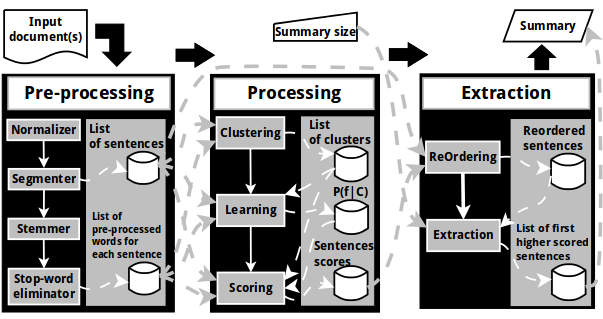
\includegraphics[width=.75\textwidth]{figures/tcc/gnrl-arch.pdf}
	\end{center}
	\caption{\label{fig:gnrl-arch} General architecture of AllSummarizer (TCC method).}
\end{figure}

\subsection{Preprocessing}

This is the language-dependent part, which can be found in many information retrieval (IR) works. 
It is needed by the method but does not affect the fact that the method is language independent. 
Also, these tools are not difficult to be found for most languages since they are simple compared to other natural language processing tasks.
In our system, we are interested in these preprocessing tasks: Normalization, Segmentation, Stemming and Stop words removal.

\subsection{Processing}

Each text contains many topics, where a topic is a set of sentences having some sort of relationship between each other.
In our case, this relationship is the cosine similarity between each two sentences. 
To generate topics, we use a simple algorithm which is based on cosine similarity and a clustering threshold $ th $ to clustering $ n $ sentences.
The sentences having a similarity greater than $ th $ are regrouped into the same cluster. 
A sentence can belong to many clusters at once, this is motivated by the fact that a sentence can discuss many topics.


A summary is a short text that is supposed to represent most information in the source text, and cover most of its topics.
Therefore, we assume that a sentence can be in the summary when it is most probable to represent all topics (clusters)  using a set of features.
So, the score of a sentence $ s_i $ is the product over classes and features of its score in a specific class and feature (see Equation. \ref{eq:globalscore}).
%
\begin{equation}
\label{eq:globalscore}
Score(s_i , \bigcap_{j} c_j , F) =  %\propto 
\prod_{j} \prod_{k} Score(s_i , c_j , f_k )
\end{equation}

The score of a sentence $ s_i $ in a specific cluster $ c_j $ and feature $ f_k $ is the sum of probability of the feature's observations when $ s_i \in c_j $ (see Equation. \ref{eq:score}).
We add one to the sum, to avoid multiplying by a features' score of zero.
%
\begin{equation}
\label{eq:score}
Score(s_i , c_j , f_k ) = 1 + \sum_{\phi \in s_i} {P(f_k=\phi | s_i \in c_j)}
\end{equation}
%
Where $ \phi $ is an observation of the feature $ f_k $ in the sentence $ s_i $.
For example, assuming the feature $ f_{k1} $ is term frequency, and we have a sentence: ``\textit{I am studying at home.}".
The sentence after preprocessing would be: $ s_i $ = \{``\textit{studi}"(stem of ``study"), ``\textit{home}"\}.
So, $ \phi $ may be ``\textit{studi}" or ``\textit{home}", or any other term.
If we take another feature $ f_{k2} $ which is sentence position, the observation $ \phi $ may take 1st, 2nd, 3rd, etc. as values.

We use 5 statistical features to score the sentences: unigram term frequency (TFU), bigram term frequency (TFB), sentence position (Pos) and sentence length (Rleng, PLeng).
We treat this features as categorical even if they are numerical. 
Thus, we will consider each 
For example, if we have a text written just with three characters: a, b and c, and the feature is the characters of the text, then we will have three categories.
Each category has a probability to occur in a cluster, which is the number of its appearance in this cluster divided by all cluster's terms, as shown in Equation \ref{eq:likelihood}. 
%
\begin{equation}
\label{eq:likelihood}
P_{f}(f = \phi | c_j) = \frac {|\{ \phi \in c_j \}|}{\sum_{c_l \in C}{| \{ \phi' \in c_l \} |}}
\end{equation}
Where $ f $ is a given feature.
$ \phi $ and $ \phi' $ are observations (categories) of the feature $ f $ .
$ C $ is the set of clusters.

\subsection{Extraction}

To extract sentences, we reorder them using their scores in decreasing order.
Then, we extract the first non similar sentences until we get the wanted size.
The next sentence to be added is compared to the last one accepted to the summary in order to decrease similarity between summary's sentences.
The logic behind this method is to select the most relevant sentences with less redundancy.

\subsection{MultiLing'15 evaluation}

These experiments have been held upon our participation in MultiLing'15 workshop \citep{15-aries-al}. 
We participated in all proposed languages, either in single document or multi-document tasks.
Contrary to our system, there are some which participated to a subset of the proposed languages. 
To compare our system against them, we followed these steps (for every evaluation metric): 
\begin{itemize}
	\item For each system, calculate the average scores of all used languages.
	\item For our system, calculate the average scores of used languages by others. 
	For example, BGU-SCE-M team uses Arabic, English and Hebrew; 
	We calculate the average of scores of these languages for this system and ours.
	\item Then, we calculate the relative improvement using the averages $ \frac{our system - other system}{other system} $.
\end{itemize}
Compared to other systems, it affords fair results, but more improvements have to be done in the future.
%This method will be used as a baseline in our next methods' experiments.




\section{Graph-based cumulative scores for multilingual ATS}

Our intention is to create a language and domain independent extractive ATS method.
Statistical and graph-based approaches are the only ones that allow us that. 
So, we try to fuse them into the method illustrated in Figure \ref{fig:archi}.
\begin{figure}[ht]
	\centering
	\includegraphics[width=.5\textwidth]{figures/gc/archi.pdf} % % %[width=140mm]
	\caption{General architecture.}
	\label{fig:archi}
\end{figure}

First the input text is preprocessed, segmenting it into sentences, which are tokenized into words, removing stop words and stemming the remaining ones. 
This is the only language-dependent part which does not pose a problem since much of its resources are available for many languages. 
Then, a graph of sentences is constructed using their similarities, which is simplified to exclude weak sentences or links. 
To score each sentence, we use statistical features then we exploit the links between sentences to enhance their scores. 
Finally, we extract the first scored sentences trying to increase summary pertinence, to decrease redundancy and to keep coherence between a sentence and the next one.

\subsection{Candidate sentences generation}

Like most graph-based works, we use cosine similarity between sentences to construct a graph $ G(V, E) $, where the nodes $ V $ represent sentences and an arcs $ E $ between two sentences is the similarity between them. 
The graph can be used to exclude some sentences from the scoring function, this will relieve the processing phase in case of a big input text. 
In our work, we try to exclude those sentence with weak relations (in number and weight) and delete weak links as well. 
Like \citet{04-erkan-radev}, we use a threshold to decide which arc to delete, but slightly different. 
The threshold is used to decide which node to remove as well.

An insignificant node, in our case, is a node which can not accumulate a total similarity weight more than one divided by the number of its important neighbors. 
Where the important neighbors $ MImpN(v_i) $ of a node $ v_i $ are defined as the ones with a similarity greater than a given threshold.
Equation \ref{eq:node-sign} represents weakness test of a given node $ v_i $, which takes boolean values: true if the node is to be deleted and false otherwise.
\begin{equation}
weak\_node(v_i) = ( \sum_{(v_i, v_j) \in E} w_{ij} < \frac{1}{MImpN(v_i)} )
\label{eq:node-sign}
\end{equation}

Since we want to use graph arcs in the scoring function, it is important to delete the weaker ones which can affect this task. 
Using the last threshold, we try to distribute it uniformly on different important neighbors of a given node to have a cutting value.
If an arc's weight is less than this value, it will be deleted. 
We should point out that, using this method, the graph will be directed; A node can consider another as a neighbor while the second one does not.
To formulate the task, Equation \ref{eq:arc-sign} represents weakness test (true or false) of an arc $ (v_i, v_j) \in E$ having a weight $ w_{ij} $.
\begin{equation}
weak\_arc(v_i, v_j) = ( w_{ij} < \frac{Threshold}{MImpN(v_i)} )
\label{eq:arc-sign}
\end{equation}

\subsection{Sentence statistical features (SSF) score}

The first step in our method is to score each candidate sentence using some statistical features, which allows the assessment of how much a sentence is pertinent towards the main topic. 
In a multilingual context, these features must be language independent. 
This is why we choose to use four features: its similarity to other candidates, the terms it contains, its size and its position in the text. 
Every feature of these four can be applied to any given language without being forced to adjust the algorithm (given the preprocessing task of this language, of course).

The first feature is sentence's cosine similarity with other candidate sentences. 
It just calculates the similarity (cosine) between a candidate sentence $ s_i $ and the remaining candidates $ C\backslash s_i $ as shown in Equation \ref{eq:ssf-sim}.
\begin{equation}
Score(s_i/ sim) = sim(s_i, C\backslash s_i)
\label{eq:ssf-sim}
\end{equation}

The second feature is term frequency which is the most famous statistical feature of all. 
To score a sentence $ s_i $ based on term frequency, we use TF-ISF.
This concept ISF is calculated as in Equation \ref{eq:isf}, where $ |C| $ is the number of candidate sentences, and $ |\{s | t \in s \wedge s \in C \}| $ is the number of candidate sentences containing this term.
\begin{equation}
isf(t) = \log \frac{|C|}{|\{s | t \in s \wedge s \in C \}|}
\label{eq:isf}
\end{equation}
We use the Euclidean normalization of its terms' TF-ISF, following the same formula used by \citet{04-nobata-sekine}. 
Equation \ref{eq:ssf-tfisf} represents the TF-ISF score of a sentence $ s_i $ given its words (terms) $ w_{ik} $.
\begin{equation}
Score(s_i/ \tfisf) = \sqrt{\sum\limits_{w_{ik} \in s_i} (\tfisf(w_{ik}))^2}
\label{eq:ssf-tfisf}
\end{equation}

The third feature is sentence size (length) which is the number of useful terms in a sentence. 
Sentence size is used to penalize short sentences since they do not carry much information \citep{95-kupiec-al}.
In our case, we do the inverse: we favor short sentences over long ones. 
Using term frequency to score sentences, a short one will not score much anyway; 
But if it does, it means that the sentence is both informative and compressed.
This score is calculated by dividing 1 on the sentence's size, as shown in Equation \ref{eq:ssf-size}.
\begin{equation}
Score(s_i/ size) = \frac{1}{|s_i|}
\label{eq:ssf-size}
\end{equation}

The last score is sentence position in the input text, used in \citep{58-baxendale,69-edmundson}.
It is based on the assumption that important sentences tend to appear at first and last. 
We follow the same method used in \citep{04-nobata-sekine}, as shown in Equation \ref{eq:ssf-pos} where $ |D| $ is the number of sentences in the input document.
\begin{equation}
Score(s_i/ pos) = \max (\frac{1}{i}, \frac{1}{|D| - i + 1})
\label{eq:ssf-pos}
\end{equation}

We consider the previous scores as probabilities of a sentence belonging to the summary. 
%Technically speaking, the scores can exceed 1 and need to be normalized in order to be used as probabilities. 
%But since the final score is used to reorder sentences, we can omit this operation (the denominator when normalizing will be the same in all sentences thus a constant). 
So, given a set of statistical features $ F = \{ sim,\ tf-isf,\ size,\ pos \} $, the overall score which we call SSF (sentence statistical features) is expressed in Equation \ref{eq:ssf}.
Assuming independence between the different features, the overall probability is the multiplication features probabilities.
% 
\begin{equation}
SSF(s_i/ F) = \prod_{f_i \in F} score(s_i/f_i)
\label{eq:ssf}
\end{equation}


\subsection{Graph-based cumulative (GC) score}

Sentence score based on statistical features such as term frequency, similarity to the text, sentence length and position can capture its pertinence towards the main subject, but does not use its relation with other sentences.
We believe exploring similarity relations among sentences can improve their scores.
On the contrary of previous graph-based methods \citep{04-mihalcea-tarau,04-erkan-radev}, our method does not exploit the concept of eigenvector centrality between connected sentences. 
Instead, it intends to improve sentence's own score (SSF) based on its neighbors by using either their scores or their amount, thus the name graph-based cumulative score (GC).
To this end, we propose four variants of GC score: GC1, GC2, GC3 and GC4. 

The first variant takes in consideration both node's and its neighbors' SSF scores, and also their similarities.
The intuition behind this variant is that a sentence can share some of its information with its neighbors. 
But, it must not share the same amount for all of them; So the similarity with a given neighbor can be used as a sharing weight (percentage).
%If the sentence is connected to important ones, this will boost its score even if it was not important. 
%The advantage of this variant is to give less scored sentences another chance, and not over-scoring them by controlling the amount of accumulation using the similarities as weights.
So, given a sentence $ s_i $ and a set of neighbors $ s_j $, the $ GC1 $ score is given in Equation \ref{eq:gc1}.
\begin{equation}
GC1(s_i) = SSF(s_i) + \sum\limits_{(s_i, s_j) \in E} sim(s_i, s_j) * SSF(s_j)
\label{eq:gc1}
\end{equation}

The second variant sums all the neighbors' SSF scores, then subtract all non-neighbors' ones.
The intuition about this variant is the same as the first one: exporting information to the neighbors. 
But in this one, the sentence is awarded for its neighbors by accumulating their scores and penalized for not being connected to other candidates.
Equation \ref{eq:gc2} represents the $ GC2 $ score of a sentence $ s_i $ given its neighbors and non-neighbors.
\begin{equation}
GC2(s_i) = SSF(s_i) + \sum\limits_{(s_i, s_j) \in E} SSF(s_j) - \sum\limits_{(s_i, s_j) \notin E} SSF(s_j)
\label{eq:gc2}
\end{equation}

A big number of neighbors is a good sign that a sentence is representative, hence it discusses topics covered by many other sentences \citep{97-salton-al}.
So, a sentence with many neighbors must score higher. 
In this variant, the score is amplified by the number of the neighbors plus one (the number of connected nodes). 
Equation \ref{eq:gc3} represents this variant where $ |\{(s_i, s_j) \in E\}| $ is the number of te neighbors of the node $ s_i $.
\begin{equation}
GC3(s_i) = SSF(s_i) * (1 + |\{(s_i, s_j) \in E\}|)
\label{eq:gc3}
\end{equation}

The last variant favorites sentences  with much neighbors' similarities. 
Each sentence is scored by its initial score multiplied by the sum of its neighbors' similarities. 
In Equation \ref{eq:gc4}, there are two possibilities: when $ a = 0 $ (lets call it $ GC4 $) and when $ a = 1 $ (lets call it $ GC5 $). 
In case of $ GC4 $, each sentence can be rewarded if the sum of similarities is more than 1, or penalized otherwise. 
The other case $ GC5 $ does not decrease the initial score, and just rewards for the amount of similarities.
\begin{equation}
GC4(s_i) = SSF(s_i) * ( a + \sum\limits_{(s_i, s_j) \in E} sim(s_i, s_j)) \text{ where } a \in \{0, 1\}
\label{eq:gc4}
\end{equation}


\subsection{Summary extraction methods}

When scoring, mostly, similar sentences will have almost the same score. 
In this case, extracting the first scored ones is not a good strategy since they may contain the same information. 
Information redundancy is one of ATS challenges; It can affect even informativeness when the summary's size is limited.
Some works incorporate redundancy management in the score itself, which is the case of the famous MMR work \citep{98-carbonell-goldstein}. 
Others try to handle redundancy after scoring, by reordering them using their original positions \citep{99-mckeown-al,00-radev-al,02-lin-hovy}, or by exploring the similarity measure between sentences \citep{15-aries-al}.

%Coherence 
Coherence is another issue since sentences must be reordered in order to give a more smooth summary. 
In our case, we want to investigate the impact of redundancy removal and sentences reordering on generated summaries. 
So, we propose six variants of extraction method, where the first selected sentence is the highest scored according to each variant.
We will express these extraction methods based on: the next sentence to be added to the summary ($ \nextsent $), a function affording the sentence which maximize/minimize a score ($ \arg\max $/$ \arg\min $), the score using a variant of our scoring method ($\ssfgc(s_i) $), similarity between two sentences ($ \simil $ ), the last sentence added to the summary ($ \lastsent $), and the descending/ascending order ($ \ord $/ $ \iord $) based on a given score.

To test how good an extraction method is, we must compare it to the standard one  ($ e_0 $).
Here, we extract the first scored sentences till reaching summary size, with no redundancy management and no coherence consideration.
So, the next sentence to be added to the summary using this method ($\nextsent_{e0}$) is the one having the highest score ($ \ssfgc $) among candidate sentences minus those already in the summary ($ C\backslash S $).
This is formulated in Equation \ref{eq:e0}. 
\begin{equation}
\begin{aligned}
\nextsent_{e0} & = & \arg\max\limits_i \ssfgc(s_i) 
\text{ where } s_i \in C\backslash S \\
\end{aligned}
\label{eq:e0}
\end{equation}


We borrowed the extraction method used in \citep{15-aries-al} which tries to manage redundancy after scoring.
The sentences are reordered using their scores; Then every time we want to add a sentence to the summary, it must be compared to the last added one.
If it is similar based on a threshold, we pass to the next sentence.
So, the next sentence to be added to the summary using this method ($\nextsent_{e1}$) is the one ($s_i$) having the highest score ($ \ssfgc $) among candidate sentences minus those already in the summary ($ C\backslash S $).
But in order to be added, it has to be less similar to the last one added to the summary ($\lastsent_{e1}$) based on a similarity measure ($\simil$) and a given threshold ($Th$).
Equation \ref{eq:e1} formulates how a sentence is selected for the summary using extraction method $e1$.
\begin{equation}
\begin{aligned}
\nextsent_{e1} & = & \arg\max\limits_i \ssfgc(s_i)
\text{ where } s_i \in C\backslash S \text{ and } \simil(s_i, \lastsent_{e1}) < Th\\
\end{aligned}
\label{eq:e1}
\end{equation}

In the third one ($ e_2 $), we try to exploit the graph structure which affords coherence information between sentences.
Sentences of the same paragraph shares some terms among themselves, since they discuss the same idea.
We want to extract the highest scored sentences which have some links between them in the graph.
Maybe, this strategy will ensure informativeness and coherence, but it is highly probable to increase redundancy. 
This is because highly scored sentences can be very similar since the scoring function uses similarity to the input text as a feature.  
So, the next sentence to be added to the summary using this method ($\nextsent_{e2}$) is the one ($s_i$) having the highest score ($ \ssfgc $) among the neighbors of the latest one previously added to the summary ($\lastsent_{e2}$) in the graph $ G(V, E) $.
Where, $ V $ is the nodes (sentences) and $ E $ is the arcs (similarity between sentences). 
Equation \ref{eq:e2} is a formulation of this variant.
\begin{equation}
\begin{aligned}
\nextsent_{e2} & = & \arg\max\limits_i \ssfgc(s_i)  
\text{ where } (\lastsent_{e2}, s_i) \in E \\
\end{aligned}
\label{eq:e2}
\end{equation}

The fourth variant ($ e_3 $) is a bit odd, proposed to test the case where we try to extract the most similar neighbors.
That is, we want to extract the neighbor with a high score (which is fine), and a high similarity which will result in high redundancy.
Insuring a high similarity between consecutive sentences in a summary does not mean it will be coherent. 
Equation \ref{eq:e3} is a formulation of this variant.
First, we extract the list of the neighbors ($s_i$) of the last added sentence to the summary ($\lastsent_{e3}$) in the graph $ G(V, E) $.
Where, $ V $ is the nodes (sentences) and $ E $ is the arcs (similarity between sentences). 
Then, we order all these neighbors' scores ($\ssfgc$) in descending order. 
Also, we order their similarities scores ($\simil$) in descending order. 
Let $ \iord $ a function that gives the ordinal of a given element in a descending ordered list.
So, the next sentence to be added to the summary using this method ($\nextsent_{e3}$) is the one ($s_i$) with the minimum descending ordinal using the score ($\iord\ssfgc$) and using similarity with the last added sentence to the summary ($\iord\simil$).
\begin{equation}
\begin{aligned}
\nextsent_{e3} & = & \arg\min\limits_i (\iord\ssfgc(s_i) + \iord\simil(\lastsent_{e3}, i)) \\
&& \text{ where } (\lastsent_{e3}, s_i) \in E \\
\end{aligned}
\label{eq:e3}
\end{equation}

The fifth variant ($ e_4 $) tries to keep the high scored neighbors with less similarity. 
Taking sentences with high score ensures the informativeness of the summary. 
Whereas selecting low similar ones will guarantee diversity and thus non redundancy. 
Even with low similarity, the chosen sentences are connected and therefore have the same context, which gives a certain level of coherence to the resulted summary.
Equation \ref{eq:e4} is a formulation of this variant.
First, we extract the list of the neighbors ($s_i$) of the last added sentence to the summary ($\lastsent_{e3}$) in the graph $ G(V, E) $.
Where, $ V $ is the nodes (sentences) and $ E $ is the arcs (similarity between sentences). 
Then, we order all these neighbors' scores ($\ssfgc$) in a descending order. 
Also, we order their similarities scores ($\simil$) in an ascending order. 
Let $ \iord $ be a function that gives the ordinal of a given element in a descending ordered list, and $ \ord $ a function that gives the ordinal of a given element in a ascending ordered list.
So, the next sentence to be added to the summary using this method ($\nextsent_{e4}$) is the one ($s_i$) with the minimum descending ordinal using the score ($\iord\ssfgc$) and the minimum ascending ordinal using similarity with the last added sentence to the summary ($\ord\simil$).
\begin{equation}
\begin{aligned}
\nextsent_{e4} & = & \arg\min\limits_i (\iord\ssfgc(s_i) + \ord\simil(\lastsent_{e4}, i)) \\
&& \text{ where } (\lastsent_{e4}, s_i) \in E \\
\end{aligned}
\label{eq:e4}
\end{equation}

The last one ($ e_5 $) seeks to keep the highest scored sentences among the neighbors which have a high amount of non-summary neighbors. 
To achieve this we extract the list of the neighbors ($s_i$) of the last added sentence to the summary ($\lastsent_{e3}$) in the graph $ G(V, E) $.
Where, $ V $ is the nodes (sentences) and $ E $ is the arcs (similarity between sentences).
These neighbors are ordered using their scores ($\ssfgc$) where $\iord\ssfgc$ is their ordinal in descending order.
So, the next sentence to be added to the summary using this method ($\nextsent_{e5}$) is the one ($s_i$) with the most non summary neighbors number ($|\{ s_j | (s_i, s_j) \in E \text{ and } s_j \notin S \}|$) and the minimum descending ordinal using the score ($\iord\ssfgc$).
This is illustrated in Equation \ref{eq:e5}.
\begin{equation}
\begin{aligned}
\nextsent_{e5} & = & \arg\max\limits_i \frac{|\{ s_j | (s_i, s_j) \in E \text{ and } s_j \notin S \}|}{\iord\ssfgc(s_i)} \\
&& \text{ where } (\lastsent_{e5}, s_i) \in E \\
\end{aligned}
\label{eq:e5}
\end{equation}


\subsection{Experiments}

To test our method, we used a corpus from MultiLing'15 workshop which contains documents and their summaries for 38 languages.
First, we tried to estimate which threshold can we use to decide if a sentence is similar to another. 
In this corpus, we found that the mean between sentences similarities gives fair results for most languages. 
Then, we selected for each scoring method an extraction strategy that maximizes its informativeness. 
After fixing all parameters, we tested our method variants against some baseline systems of well known ATS methods. 
Our method did a good job especially $ GC1 $ variant with $ e4 $ scoring method, either in term of recall or precision.
GC1 variant gives better informativeness (recall) because it cumulates scores from sentence's neighbors weighted by their similarities. 
A sentence that shows high similarities to its neighbors should score better. 
Also, a high connected one is more probable to discuss the main topic of the input text. 
In addition to the number of neighbors and similarity, a sentence connected to high scored neighbors is more likely to be important. 
High precision can be explained by the use of extraction method $ e4 $. 
It tries to set a trade-off between informativeness and redundancy: maximize the score and minimize the similarity. 
Also, it extracts connected sentences in the graph to guarantee some coherence. 



\section{(ML)$_\text{2}$ExtraSum: Machine Learning based Multi-Lingual Extractive Summarizer}

Our idea is to express the problem of text summarization as a problem of regression. 
Using some features of a sentence and its document, the system must learn to estimate ROUGE-1 of this sentence based on a reference summary. 
As shown in Figure~\ref{fig:ml2extrasum-archi}, we build some blocks of multi-layer neural networks which we call scorers. 
Each scorer receives one type of features; for instance, there is a scorer which scores a sentence based on its term frequencies and those of its document. 
All these scorers outputs are fed into another scorer to be combined into one final score which is meant to be an estimation of ROUGE-1 score of the sentence in question. 
The system is trained on multiple languages, this is why a block (language clusterer) is reserved to detect the language.
In our case, the language clusterer represent each language as a two dimensional vector which is fed into other scorers so they learn to score based on the language. 
\begin{figure}[ht]
	\centering
	\includegraphics[width=.5\textwidth]{figures/ml2extrasum/archi.pdf} % % %[width=140mm]
	\caption{General architecture of ML2ExtraSum.}
	\label{fig:ml2extrasum-archi}
\end{figure}

We use two types of features based on their mathematical representations: 
\begin{itemize}
	\item \textbf{Vector representations}: a sentence or a document is represented by a vector of values. 
	The features represented as vectors are: \textit{doc\_tf\_seq}, \textit{doc\_sim\_seq}, \textit{doc\_size\_seq}, \textit{sent\_tf\_seq} and \textit{sent\_sim\_seq}.
	\item \textbf{Scalar representations}: a sentence or a document is represented by one value. 
	The features represented as scalars are: \textit{nbr\_sents}, \textit{sent\_size} and \textit{sent\_pos}.
\end{itemize}

\subsection{Basic model}

In this model, we use the features as they are without any transformation. 
Nevertheless, in our experiments we limit the number of sequences to 50 by keeping only the highest values among them. 
These sequences are ordered then fed into LSTM cells to transform these sequences into one score.
%Figure~\ref{fig:ml2extrasum-basic} represents our basic model components (the sentence scorer was explained earlier in Method overview).
%
%\begin{figure}[!ht]
%	\centering
%	\begin{tabular}{cc}
%		\includegraphics[height=.2\textwidth]{figures/ml2extrasum/basic-a.pdf}
%		&
%		\includegraphics[height=.2\textwidth]{figures/ml2extrasum/basic-b.pdf}
%		\\
%		(a) Language clusterer & (b) TF or Similarity scorer\\
%		\includegraphics[height=.2\textwidth]{figures/ml2extrasum/basic-c.pdf}
%		&
%		\includegraphics[height=.2\textwidth]{figures/ml2extrasum/basic-d.pdf}
%		\\
%		(c) Position scorer & (d) Size scorer \\
%	\end{tabular}
%	
%	\caption{Components of the basic model of ML2ExtraSum.}
%	\label{fig:ml2extrasum-basic}
%\end{figure}

\subsection{With filtering}

This one has the same architecture as the previous variant. 
The only difference is filtering the sequences: \textit{doc\_tf\_seq}, \textit{doc\_sim\_seq}, \textit{doc\_size\_seq}, \textit{sent\_tf\_seq} and \textit{sent\_sim\_seq} before feeding them into the system. 
For each sequence, the system uses just the values higher than the mean. 
This will reduce the working space and will help the system focusing on the most important values.

\subsection{With normalization and filtering}

Normalizing the values helps the system converging faster. 
The architecture stays the same as the basic one; the only difference is in Features transformation step. 
This is a list of features and the transformation functions applied to them:
\begin{itemize}
	\item We apply a min-max normalization then a filtering function on: \textit{doc\_tf\_seq}, \textit{doc\_size\_seq} and \textit{sent\_tf\_seq}. 
	The min and max values are the calculated from the document. 
	For example, to normalize \textit{doc\_tf\_seq} or \textit{sent\_tf\_seq} both take the maximum TF in the document as max and the minimum tf in the document as min.
	\item We apply a filtering function on: \textit{doc\_sim\_seq} and \textit{sent\_sim\_seq}. 
	Their values are known between 0 and 1, therefore no need to normalize.
	\item The scalar \textit{sent\_size} is normalized, where \textit{max} (\textit{min}) is the maximum (minimum) size of sentences in the document.
\end{itemize}
The scalar \textit{doc\_size} is not normalized since the training batch is a document. 
Also, \textit{sent\_pos} is not normalized since it is used with \textit{doc\_size}.

\subsection{With scalar features}

In this version, we want to use just scalar features (no sequences) and create new features as well. 
Then, each type of features is fed into its related scorer as an input layer. 
The intermediate scorers, in this version, have all just one layer of 50 perceptrons. 
They have one output, expect of language clusterer which has two. 
%Figure~\ref{fig:ml2extrasum-pure} shows the new created features using the transformation functions we presented earlier.
%The new size features are based on min and max clipping, where the minimum and maximum limits are calculated from document's sizes by weighting the mean and the max sizes. 
%The weights we used in our system are: $ \alpha 1 = 0.7 $, $ \alpha 2 = 1.3 $, $ \beta 1 = 0.3 $ and $ \beta 2 = 0.7 $.
%%
%\begin{figure}[!ht]
%	\centering
%	\includegraphics[width=\textwidth]{figures/ml2extrasum/pure.pdf} % % %[width=140mm]
%	\caption{New scalar features created using transformation of the old ones.}
%	\label{fig:ml2extrasum-pure}
%\end{figure}

\subsection{Experiments}

To test our system, we used AllSummarizer\_TCC \citep{13-aries-al,15-aries-al}, which does not use machine learning at all, as a baseline system. 
Unfortunately, ML2ExtraSum had no chance against AllSummarizer\_TCC in any of its variants. 
This tells us that our ML based architecture maybe needs more than some surface features to reach its full potential. 
Another assumption is that ML is not as fit to score the pertinence of a sentence in a multi-lingual context as a traditionally encoded solution based on observation does. 
At least, not in the way our architecture is proposed. 

We must, also, take in consideration that the training batch was a document. 
So, if the whole dataset was used as a batch, result might be different.
Letting the system extracting the features by itself such as using word embedding is interesting, but it will require sacrificing the multi-lingual aspect of the system. 
Moreover, it will consume a lot of data to construct a valid vocabulary. 


\section{Conclusion}

A literature review has been presented to introduce ATS especially in multilingual context.
After introducing ATS, a brief description on our participation in MultiLing'15 workshop has been presented. 
Then, a section is reserved for our new method which combines surface features with graphs approach in order to score sentences. 
After that, we presented another method we proposed using machine learning and statistical features to extract sentences.

In conclusion, multilingual automatic text summarization is an important domain nowadays.
It can help professionals processing the huge information overload due to the increase rate of multilingual web content.
In this case, the more a system uses language-independent resources, such as toolkits and corpora, the more it can adapt to new languages. 

\subsection{Contributions}

% Informativeness 
Informativeness is the most important indicator of a good summary.
In this thesis, we tried to maximize the quantity of information a summary can contain whatever the language of the original text. 
First of all, we enhanced our previous method (TCC) \citep{13-aries-al} and tested it in a multilingual context by participating in MultiLing'15 workshop \citep{15-aries-al}.
The method, being tested and proved its quality, has been used as a baseline to test our new method (SSF-GC). 
The new method called ``Sentence statistical features, Graph-based cumulative scores" (SSF-GC) combines surface features and similarity graph to score sentences, as indicated by its name. 
The graph is used to exclude some sentences which have week links with others, thus they are off-topic and less informative. 
We can consider this step as a noise removal task to enhance the scoring function. 
The informativeness of each sentence is expressed as its probability to belonging to the summary based on some statistical features. 
In our case, this probability is affected by the sentence's neighbors' in the graph using accumulation.
We proposed some scoring functions which gave good results.
Our machine learning based method (ML2ExtraSum) could not beat TCC method in term of informativeness. 
Nevertheless, it affords close results and it can be a good start to be enhanced in the future.


% Redundancy 
Redundancy is another issue in ATS. 
Unlike MMR \citep{98-carbonell-goldstein} which tries to handle informativeness and redundancy using one score, we treat redundancy while extracting sentences. 
This separation gives us more freedom on how we extract relevant sentences based on their informativeness scores, but using some conditions to decide if the summary has already the information in a sentence about to be extracted. 
A first attempt was to use similarity between the last sentence added to the summary and the next one being considered for the summary. 
If there is a huge similarity between them, we consider another sentence. 
This extraction method has proven to be a good one. 
It does not just improve non redundancy, but also informativeness by letting the space for more new information. 
We tested using other variants, mostly based on the graph. 
One variant, in particular, gives good results. 
It is similar to the one we described earlier, but it is based on the graph. 
First, we choose the highest scored sentence among the candidates. 
Then, out of its neighbors, we choose the one which maximizes the score and minimizes the similarity.  

% Coherence
Also, we tried to propose some extraction methods with coherence in mind. 
Mostly, a paragraph's sentences have some shared terms, especially the consecutive one. 
So, when we order sentences, it is natural that a sentence following another has some similarity. 
But, this similarity must not exceed some limit, otherwise it will be a repetition. 
Unfortunately, we did not test how far this assumption is true, and how to define such limit.

% delivrables 
Aside from the theoretical contributions, this thesis contributes to the state of art by making tools available to the community. 
We designed some open source tools to support this thesis; the most important are these two which we talked about earlier in this thesis:
\begin{itemize}
	\item \textbf{AllSummarizer}: A Java platform for extractive text summarization. 
	It implements the two methods discussed here, in this thesis \citep{13-aries-al,15-aries-al}.
	It has three parts: preprocessing, processing and postprocessing. 
	More information about the system is presented in Appendix A.
	
	\item \textbf{LangPi}: a Java tool for preprocessing: Normalization, Segmentation, Stemming and Stop words removal.
	The tool affords ROUGE metrics for summarization which support multilingual evaluation. 
	
	\item \textbf{ML2ExtraSum}: a Python tool for extractive text summarization based on machine learning using Tensoflow. 
	Along with it, a preprocessed corpus based on MultiLing'15 MSS corpus.
	
\end{itemize}

\subsection{Limits}

% simplicity
In our work, we tried to propose a method for multilingual ATS which is simple yet effective.
In the end, simple things are not always bad;  like Leonardo da Vinci said: ``Simplicity is the ultimate sophistication.".
However, usually complex tasks such as ATS demand complex mechanisms. 
In SSF-SG method, we assumed the different features scores are probabilities and combined them accordingly.
This assumption gave good results, yet it does not mean there are no better combinations. 
Although we had to avoid machine learning due to language dependency, we decided to test using this approach in our method/system ML2ExtraSum. 
So, we formulated summarization task as a regression problem: estimating ROUGE-1 score from a set of features. 
The scoring function is estimated using many neural networks blocks: Language Clustering Scorer, TF-ISF Scorer, Similarity Scorer, Size Scorer and Position Scorer. 
Each of these blocks affords a score, then all these scores are fed to another block called ``Sentence Scorer" to estimate ROUGE-1 score of the sentence.
The system was trained using Multling'15 MSS training corpus and tested using the testing one. 
Unfortunately, this method did not outperform our TCC method, because the system could not estimate ROUGE-1 properly. 
%A more detailed description of this experience can be found in Appendix B.

% pertinence and redundancy
Like we said, a task such as ATS is way too complex to be expressed by a simple method. 
Surface features are good indicators on a sentence's pertinence. 
Nevertheless, they cannot express the deep meaning of sentences. 
As a consequence, a sentence can be pertinent to the general topic but the system cannot capture that; for example, if it contains synonyms of important terms.
Also, the final summary can have redundant sentences, which does not share the same terms but have the same meaning.


%% readability
Readability remains an issue of ATS. 
In our case, we tried to focus on coherence using sentences ordering. 
Unfortunately, this was not tested since it needs a lot of experts to access the order of sentences. 
Also, anaphora resolution and replacing conjunctions were not treated in our work since these operations can be seen as a post-processing task.


\subsection{Future works}

% talk about 
Our SSF-GC method affords acceptable results in the context of multilingual ATS, given the tests we performed.
However, looking at the limits we enlisted earlier, it is still far away from being a perfect one. 
Statistical surface features are good indicators of sentence pertinence.
Therefore, they afford good summaries in term of informativeness, without sacrificing the method's multilingualism.
Still, they cannot capture the whole meaning, which results in less informativeness and more redundancy. 
In this case, a more sophisticated approach is to summarize ideas in a language-independent format. 
To do this, we have to design a way to represent sentences in a general way without loosing their meanings.
This leads us to Chomsky's universal grammar which states that there is an innate language faculty, which is genetically determined, that allows children to learn a specific language \citep{80-chomsky}.
We will not discuss language acquisition theories and nativism theory criticism (although, there are neuroscience researches suggesting Chomsky may be right \citep{16-ding-al}). 
The objective is to find a representation which can satisfy a maximum number of languages, even if there are some exceptions.


If we can find a way to represent sentences meanings regardless their original language, it is not just multilingual ATS that will be improved. 
We can talk about cross-lingual summarization, which seeks to generate a summary in a language different from the original one. 
We can go further by summarizing multiple documents in many different languages into a summary with a target language.
That being said, this is not possible unless we have some language-dependent tools. 
A universal representation of the meaning can help us create multilingual methods for ATS. 
However, we have to possess the tools allowing us to pass from each natural language to this representation and vice versa. 
In the end, the problem of multilingual ATS comes back to resources' availability.


Another alternative is to exploit machine learning while trying to maintain the system's independence from the training corpus. 
To this end, we implemented a multilingual system (ML2ExtraSum) based on machine learning; but it could not surpass the baseline.
As future directions, how adding more features can affect the system's performance must be investigated.
Nowadays, there are tools that afford some deep language features for multiple languages, such as BabelNet\footnote{BabelNet website: \url{https://babelnet.org/} [27 August 2019]} \citep{12-naigli-ponzetto}.
Also, generating more new features may help the system as shown by \textit{pure} model in our experiments. 
On the bright side, the system shows promising results when it comes to clustering languages based on summarization.
Same as scoring, the task of clustering  still has to be improved so it can separate languages and represent them in a larger range.


%\section{Bibliography}

\bibliographystyle{humannat}
{\footnotesize \bibliography{references}}


\end{document}

